\documentclass[12pt,a4paper,openright,oneside]{book}
\usepackage{my-style}

\author{Andrea Acampora}

\begin{document}

\frontmatter
\title{Tesi}
\date{\today}

\newgeometry{margin=0.8in}
\begin{titlepage}
    \begin{center}

\large
\textbf{ALMA MATER STUDIORUM - UNIVERSITÀ DI BOLOGNA} \\
\textbf{CAMPUS DI CESENA} \\
\vspace{0.5cm}
\textbf{DIPARTIMENTO DI INFORMATICA -\\ SCIENZA E INGEGNERIA}\\
\vspace{0.5cm}
\Large
\textit{Corso di Laurea in Ingegneria e Scienze Informatiche} \\


\vspace{0.7cm}
\noindent\rule{\textwidth}{0.7pt}


\vspace{2.5cm}

\large{\textbf{\MakeUppercase{
Ri-progettazione del modulo di esportazione dati del simulatore Alchemist
}}}

\vspace{2cm}

Tesi di Laurea in \\
PROGRAMMAZIONE AD OGGETTI


\vspace{3cm}

\begin{minipage}[t]{7cm}
\flushleft
\textit{{Relatore}}

\textbf{Prof. Danilo Pianini}\\
\end{minipage}
\hfill
\begin{minipage}[t]{7cm}
\flushright
\textit{Presentata da}

\textbf{Acampora Andrea}
\end{minipage}

\flushleft
\textit{{Correlatore}}

\textbf{Prof. Mirko Viroli} \\

\vspace{3cm}
\noindent\rule{\textwidth}{0.7pt}
\vspace{1cm}

\centering
Anno Accademico 2020/2021
    \end{center}
\end{titlepage}
\restoregeometry



\begin{abstract}
Le simulazioni computerizzate sono uno strumento vitale utilizzato nell'analisi del comportamento di sistemi complessi.
Ad oggi le simulazioni sono diventate parte integrante dell'ingegneria dei sistemi computazionali, principalmente durante la fase di progettazione per testare, convalidare e prevedere il comportamento del sistema prima di iniziare l'effettiva fase di dispiegamento.
In generale, le simulazioni computerizzate richiedono la definizione di un modello del dominio, la sua implementazione eseguibile, l'effettiva esecuzione e la produzione dei dati di output.
L'esportazione dei dati è un aspetto chiave nel contesto delle simulazioni computerizzate, in quanto rappresenta l'output dell'operazione di simulazione.
Lo scopo di questo lavoro è quello di analizzare il dominio della generazione di dati tramite simulazione, analizzare lo stato dell'arte e infine applicare quanto appreso nella ri-progettazione di un modulo di esportazione dati per il simulatore Alchemist.
Fra gli altri, il nuovo modulo dovrà superare le limitazioni del sistema originale in termini di flessibilità e prestazioni.
\end{abstract}

\tableofcontents

\mainmatter

\chapter{Contesto e Motivazioni}

\section{Le simulazioni computerizzate}
Le simulazioni computerizzate sono uno strumento vitale utilizzato nell'analisi del comportamento di sistemi complessi.
Ad oggi le simulazioni sono diventate parte integrante dell'ingegneria dei sistemi computazionali, principalmente durante la fase di progettazione per testare, convalidare e prevedere il comportamento del sistema prima di iniziare l'effettiva fase di dispiegamento.
In generale, possiamo intendere le simulazioni computerizzate~\cite{sep-simulations-science} come un metodo per studiare sistemi. Questo metodo, o processo~\cite{comp-sim-ieee} si componde delle seguenti fasi:
\begin{enumerate}
    \item la presenza di un \textit{fenomeno} che si intende osservare;
    \item l'implementazione di un modello matematico rappresentativo del fenomeno;
    \item la trasformazione in un modello eseguibile;
    \item l'indagine del fenomeno di partenza attraverso il modello opportunamente creato. In questa fase, durante l'esecuzione della simulazione, verrà aggiornato lo stato del sistema e delle variabili presenti nel modello seguendo un opportuno criterio per lo scorrere del tempo;
    \item l'analisi delle informazioni ottenute e generate durante la simulazione.
\end{enumerate}
Le simulazioni computerizzate, inoltre, fungono da strumento pedagogico~\cite{comp-sim}. Anche quando un problema presenta una soluzione analitica, possiamo utilizzare le simulazioni per comprendere ed analizzare il processo che l'ha prodotta.
Nel corso degli anni le simulazioni computerizzate sono state responsabili di una serie di progressi e sono diventate indispensabili nella modellazione di molti sistemi sia naturali (fisica~\cite{comp-sim-phys}, chimica~\cite{comp-sim-chem}, biologia~\cite{comp-sim-biol}) che economici~\cite{comp-sim-econ} e sociali~\cite{comp-sim-soc}. 
Inoltre, le simulazioni sono ampiamente utilizzate in tutti i rami dell'ingegneria al fine di ottenere una maggiore comprensione e conoscenza dei sistemi appena menzionati.
In sintesi, le principali motivazioni~\cite{Zeigler:2000} che portano all'utilizzo delle simulazioni computerizzate sono:
\begin{itemize}
    \item In un sistema complesso non sempre è possibile trovare una descrizione analitica;
    \item Un esperimento in un contesto reale e non digitalizzato è spesso meno efficiente, più costoso, e solitamente più complesso;
    \item In molti contesti le simulazioni permettono di analizzare e comprendere un sistema reale a cui è impossibile accedere;
    \item Esistono scenari in cui vengono simulate le condizioni che portano alla distruzione di un sistema. Nella maggioranza dei casi, la distruzione di un sistema reale non è permessa e di conseguenza le simulazioni computerizzate rimangono l'unica soluzione;
    \item Alcuni esperimenti, per svariate ragioni, necessitano di poter fermare l'esecuzione. Questo aspetto è certamente possibile in una simulazione computerizzata, mentre può risultare complicato in contesti reali.
\end{itemize}

Le simulazioni necessitano di un set di dati di partenza che vengono forniti attraverso sensori e attuatori, file di configurazione, valori generati da un qualche processo oppure valori di output di altre simulazioni. 

\section{Generazione di dati tramite simulazioni}

Molte simulazioni computerizzate, a prescindere dal contesto in cui operano, generano continuamente grandi quantità di dati.
Gli utilizzi e le funzionalità~\cite{Garrido2009} dei dati generati dalle simulazioni possono essere raggruppati come segue:

\begin{enumerate}
    \item Fornire un resoconto della simulazione  effettuata e di ciò che la computazione ha generato;
    \item Valutare e confrontare le prestazioni dei modelli adottati;
    \item Nelle simulazione stocastiche, in cui sono presenti parametri stocastici, è necessario eseguire delle analisi per verificare che i valori generati siano statisticamente significativi.
\end{enumerate}

Sebbene essi siano estremamente rilevanti attualmente non è presente uno standard per l'esportazione.
Le ragioni risiedono nel fatto che i dati da esportare variano in base al dominio in cui opera la simulazione, ed essendo esse utilizzate in numerosi campi risulta impossibile adottare un formato standard che sia adeguato a tutti i contesti.
A fronte di ciò, spesso si ricorre all'utilizzo di formati personalizzati, i quali sono creati ad-hoc sul dominio dei dati che si intende esportare.

\subsection{Esempi in letteratura}
Il simulatore \textbf{Repast}~\cite{repast}, nato all'interno dell'Università di Chicago, è uno strumento open-source per la modellazione e simulazione basata su agenti. Per quanto riguarda l'esportazione dei dati il simulatore Repast permette all'utente di generare un file di testo con i dati di output e supporta inoltre la visualizzazione di essi tramite grafici.
\textbf{Neuron}~\cite{kumbhar2019coreneuron} è un simulatore utilizzato nell'ambito della neuroscienza per studiare le attività elettriche delle reti neuronali. Neuron esporta i dati in diversi file in formato \textit{High Oriented Calculator}(HOC). In particolare, genererà un file contente i soli parametri della simulazione, un file contenente i dati della simulazione ed un file da utilizzare per visualizzare grafici in 3D. \textbf{NetLogo}~\cite{netlogo}, un ambiente completo per la programmazione multi-agente, non permette un esportazione diretta dei dati della simulazione ma consente di visualizzarli tramite grafici e, solo al termine dell'esecuzione, è possibile esportare i dati dei grafici su un file in formato CSV. Il simulatore ad eventi \textbf{NS-3}~\cite{ns3}, utilizzato per scopi di ricerca nell'ambito delle reti internet, prevede un modulo di import/export che si occupa di tradurre i dati della simulazione nel formato \textit{Functional Mock-Up Interface}(FMI)~\cite{fmi}.
\textbf{Omnet++}~\cite{omnet}, una piattaforma per simulazioni ad eventi di reti internet, utilizza il formato \textit{Network Description}(NED) per la configurazione delle simulazioni. In aggiunta, per esportare i dati mette a disposizione un modulo che consente di convertire dal formato \textit{NED} al formato \textit{JSON}, in modo da agevolare la comprensione dei dati di output. 

\chapter{Il simulatore Alchemist}
\textbf{Alchemist} è un simulatore stocastico \textit{open-source} nato all’interno dell’Università di Bologna, che permette la simulazione di scenari inerenti la computazione pervasiva, aggregata ed ispirata alla natura.
\section{Analisi del modello di dominio}
Il dominio del simulatore Alchemist, rappresentato in \cref{fig:alchemist-meta-model}, è composto dalle seguenti entità:
\begin{itemize}
    \item \textbf{Molecola}: può essere associata ad un concetto di variabile in un linguaggio di programmazione imperativo. Ogni \textit{molecola} è descritta non solo da una \textit{concentrazione}, ma da un insieme di proprietà in modo che lo stato del sistema possa essere complesso e strutturato.
    \item \textbf{Concentrazione}: è il valore di una determinata \textit{molecola}. Può essere associato al valore di una variabile in un linguaggio di programmazione.
    \item \textbf{Nodo}: contenitore di \textit{reazioni} e \textit{molecole} situato all'interno di un \textit{ambiente}.
    \item \textbf{Ambiente}: rappresenta  un'astrazione dello spazio. E' un contenitore di \textit{nodi} e ha la funzione di:
    \begin{enumerate}
        \item comunicare la posizione dei nodi nello spazio.
        \item comunicare la distanza tra due nodi.
        \item funge da supporto per i nodi in movimento.
    \end{enumerate}
    \item \textbf{Regola di associazione}: una funzione di un determinato \textit{ambiente} che associa ogni \textit{nodo} ad un \textit{vicinato}.
    \item \textbf{Vicinato}: un'entità composta da un nodo e un set di nodi vicini.
    \item \textbf{Reazione}: Il concetto di \textit{reazione} è da considerarsi molto più elaborato di quello utilizzato in chimica: in questo caso, si può considerare come un insieme di \textit{condizioni} sullo stato del sistema, che qualora dovessero risultare vere innescherebbero l’esecuzione di un insieme di \textit{azioni}. La frequenza di accadimento di una reazione può dipendere dal valore di ciascuna \textit{condizione}, da un tasso statico, da una distribuzione temporale e da un'equazione che a partire dal tasso statico e dai valori delle condizioni restituisce un tasso istantaneo. (Vedere \cref{fig:alchemist-reaction} per comprendere il funzionamento). Ogni \textit{nodo} contiene un'insieme anche vuoto di reazioni. 
    \item \textbf{Condizione}: funzione booleana che prende in ingresso un ambiente e determina se una \textit{reazione} deve essere eseguita.
    \item \textbf{Azione}: modella un cambiamento nell'ambiente.
\end{itemize}
\begin{figure}
	\centering
	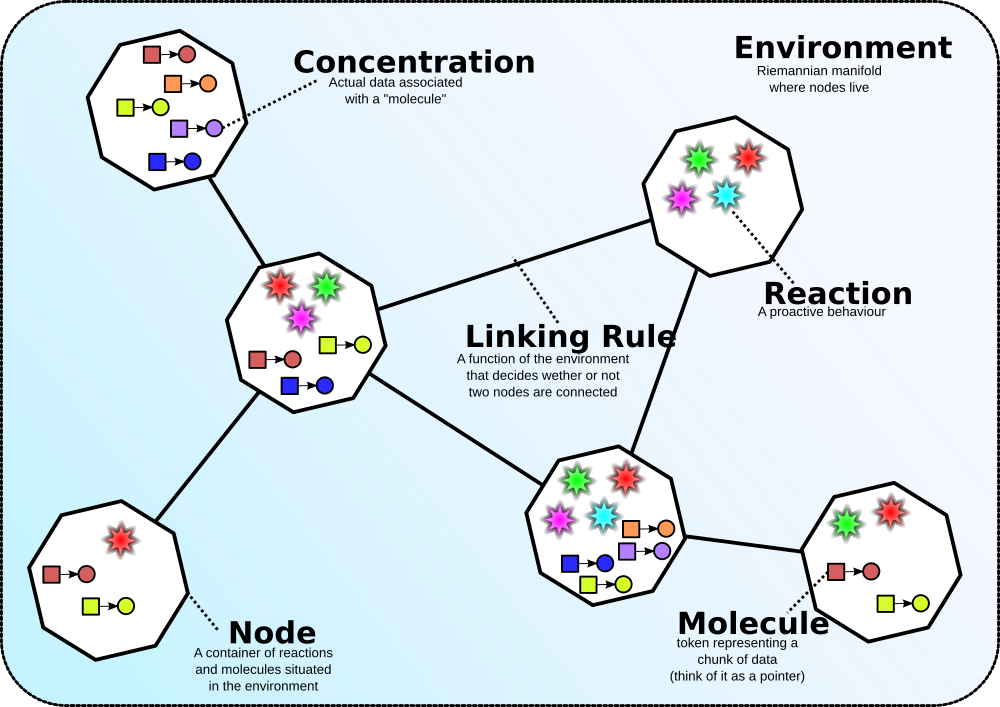
\includegraphics[width=0.8\linewidth]{images/alchemist-meta-model.png}
	\caption{Il modello computazionale di Alchemist: uno spazio continuo contenente nodi. Ciascun nodo è programmato con un set di reazioni e contiene un set di molecole. }
	\label{fig:alchemist-meta-model}
\end{figure}
\begin{figure}
	\centering
	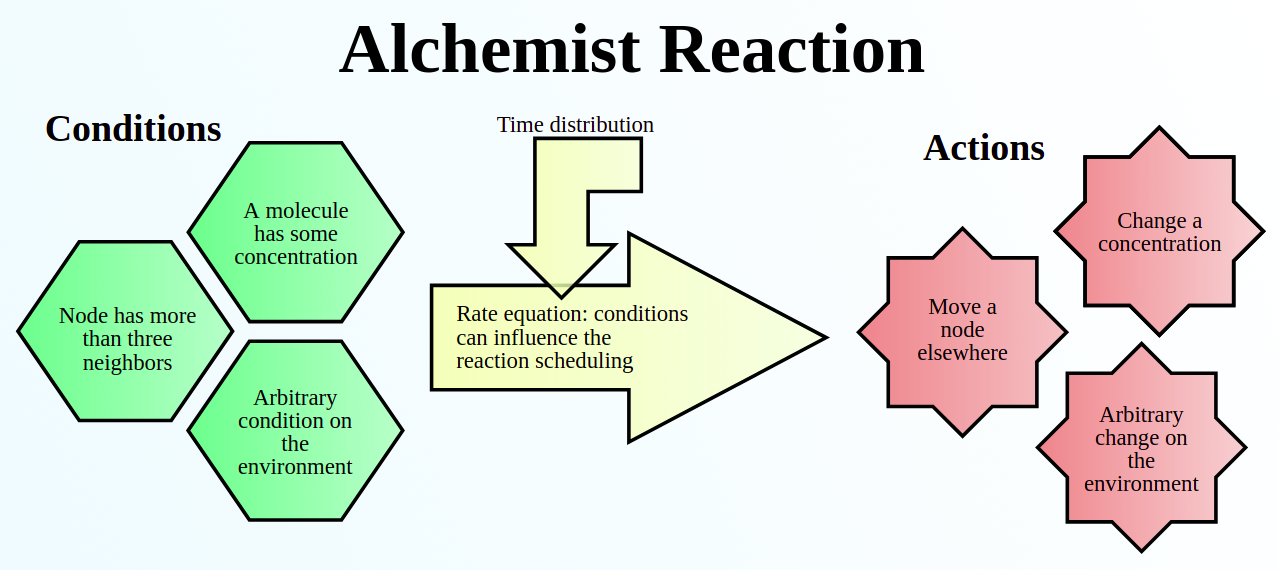
\includegraphics[width=1\linewidth]{images/alchemist-reaction.png}
	\caption{Rappresentazione grafica del funzionamento di una reazione.}
	\label{fig:alchemist-reaction}
\end{figure}
Le implementazioni del meta-modello sono definite come incarnazioni ed hanno l’obbligo di ridefinire il concetto di concentrazione delle molecole. Al momento le incarnazioni presenti sono: \textit{Protelis}, \textit{Sapere}, \textit{Biochemistry}, \textit{Scafi}.
\section{Funzionalità ed utilizzo del simulatore}
Le simulazioni in Alchemist vengono configurate all'interno di file YAML~\cite{YAML2009}, un formato per la serializzazione di dati facilmente leggibile.
Nei file di configurazione è necessario specificare quali classi e parametri utilizzare.
Le entità vengono identificate tramite chiavi, al livello zero troviamo ad esempio:
\begin{itemize}
    \item \textbf{incarnation}: l'unica chiave obbligatoria. Serve a specificare quale incarnazione si vuole utilizzare;
    \item \textbf{seed}: specifica i semi da utilizzare per la generazione di numeri casuali;
    \item \textbf{variables}: una lista di variabili aggiuntive;
    \item \textbf{environment}: la tipologia di ambiente dentro al quale svolgere la simulazione;
    \item \textbf{network-model}: permette di scegliere come devono essere collegati tra loro i nodi a seconda della classe;
    \item \textbf{export}: permette di configurare e scegliere i dati della simulazioneda esportare;
    \item \textbf{deployment}: permette di definire quali sono i nodi del sistema e dove si trovano.
\end{itemize}
Per una descrizione più dettagliata delle chiavi si faccia riferimento al sito di Alchemist\footnote{\url{https://alchemistsimulator.github.io/wiki/usage/yaml/}}.
Il simulatore può funzionare in due modalità: interattiva o batch.
Nella prima viene eseguita una sola simulazione per volta mentre in modalità batch possono essere eseguite molteplici simulazioni a seconda dei valori delle variabili impostati dall'utente.
Le variabili permettono quindi di impostare dei set di valori al posto di un valore singolo. In caso di più variabili con più valori, il simulatore
eseguirà una simulazione per ogni possibile combinazione delle stesse, ossia eseguirà un numero di simulazioni pari alla cardinalità del prodotto cartesiano delle cardinalità dei valori delle stesse.
L'elevato grado di libertà nella configurazione delle simulazioni permette ad Alchemist una serie di funzionalità, tra le quali:
\begin{itemize}
    \item l'esecuzione di programmi Scafi\footnote{\url{https://scafi.github.io/}}.
    \item l'esecuzione di programmi Protelis\footnote{\url{https://protelis.github.io/}}.
    \item l'esecuzione di programmi SAPERE\footnote{\url{https://www.unibo.it/en/research/projects-and-initiatives/Unibo-Projects-under-7th-Framework-Programme/cooperation-1/information-and-communication-technology-ict-1/sapere}}.
    \item la simulazione di ambienti bidimensionali.
    \item la simulazione di pedoni con modelli cognitivi.
    \item l'esecuzione di simulazioni in ambienti interni importando immagini in bianco e nero e ambienti esterni come mappe fornendo anche supporto alla navigazione.
    \item la simulazione di reti di smart-cameras.
    \item l'esecuzione di simulazioni in ambienti distribuiti.
\end{itemize}
\section{Riproducibilità degli esperimenti scientifici}
Un fenomeno che non può, almeno in linea di principio, essere riprodotto o osservato a piacimento non può essere materia di indagine scientifica.
Nonostante Alchemist utilizzi un modello computazionale puramente stocastico, uno dei punti chiave del simulatore è quello di garantire la riproducibilità degli esperimenti scientifici.
Nel simulatore è infatti essenziale anche a fini di debug riuscire a garantire delle simulazioni sempre uguali tra loro partendo da una stessa configurazione nel file YAML.

\section{Analisi dell'architettura di esportazione dati preesistente}
Alchemist utilizza un'architettura di tipo ECB~\cite{ECB} (\textit{Entity Control Boundary)}.\\
Il pattern architetturale ECB può essere considerato un'estensione del pattern MVC~\cite{MVC} dove le \textit{entity} corrispondono al \textit{model} ed i \textit{boundary} alla \textit{view}:
\begin{itemize}
    \item \textbf{Entity}: entità passiva, rappresentativa di una qualche parte del domonio;
    \item \textbf{Control}: funge da intermediario tra \textit{entity} e \textit{boundary};
    \item \textbf{Boundary}: incapsula le interazioni con attori esterni.
\end{itemize}

Nel pattern la responsabilità di ogni classe è associata al ruolo che assume nel diagramma dei casi d'uso, nello specifico il \textit{boundary} trasmette l'input dell'utente al controller e ne gestisce l'output mentre il controller contiene l'implementazione del motore del simulatore attraverso il quale modifica lo stato delle entità del dominio.
Il \textit{controller} comunica lo stato del sistema ai \textit{boundary} tramite l'interfaccia \texttt{OutputMonitor} per esportarlo ad una GUI oppure su file.
La \cref{fig:alchemist-ecb-arch} mostra come viene applicatto il pattern nell'architettura del simulatore Alchemist.
\begin{figure}
	\centering
	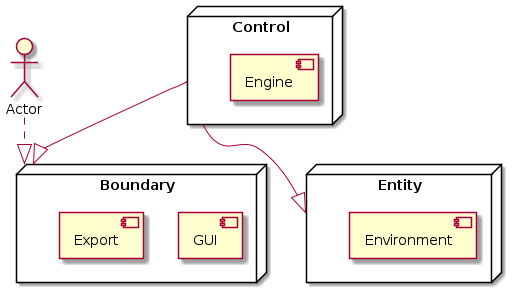
\includegraphics[width=1\linewidth]{images/alchemist-ecb.png}
	\caption{Diagramma dell'architettura ECB di Alchemist.}
	\label{fig:alchemist-ecb-arch}
\end{figure}

L'attuale sistema di Export è basato sulla scrittura dei dati della simulazione su un file di testo in formato CSV.
La classe responsabile dell'esportazione dei dati è l'\texttt{Exporter} che implementa direttamente il boundary \texttt{OutputMonitor}.
Nella fase di setup viene aggiunto all'\texttt{Engine}, ossia al \textit{Controller}, il boundary rappresentato dalla classe \texttt{Exporter}. In questo modo il controller notificherà all'\texttt{Exporter} per ogni step della simulazione i relativi dati riguardanti le reazioni avvenute e quest'ultimo provvederà ad elaborarli ed esportarli su file.
Nell'elaborazione ed estrazione dei dati l'\texttt{Exporter} utilizza l'interfaccia \texttt{Extractor}, la quale prevede una serie di implementazioni a seconda della tipologia di dato da estrarre.
Nella \cref{fig:UML_old_arch} viene mostrato il diagramma delle classi dell'architettura preesistente del simulatore Alchemist.
\begin{figure}[H]
    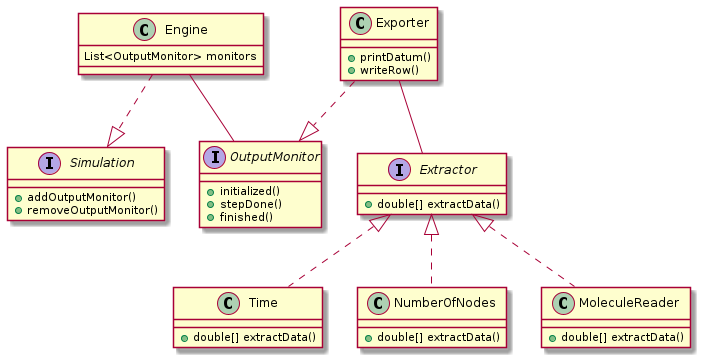
\includegraphics[width=\textwidth]{images/alchemist-export-old.png}
    \caption{schema UML della architettura di export di Alchemist esistente.}
    \label{fig:UML_old_arch}
\end{figure}
La scelta dei dati che si intende esportare avviene all'interno del file di configurazione YAML con la chiave \textit{export}. Inoltre è possibile aggiungere dei filtri e aggregatori sui dati come minimo, massimo, media, varianza come nel seguente esempio:
\begin{minted}[
    gobble=4,
    frame=single,
    linenos,
    samepage
  ]{yaml}
    export:
        - time
        - molecule: "default_module:default_program"
        aggregators: [mean, max, min, variance, median]
        value-filter: onlyfinite
        
\end{minted}
La linea di comando presenta i seguenti parametri:
\begin{itemize}
    \item \texttt{-e, -{}-export}: parametro obbligatorio se si intende effettuare la fase di export. Contiene una stringa formata dal percorso in cui verrà generato il file di output.
    \item \texttt{-i, -{}-interval}: parametro opzionale, rappresenta l'intervallo di campionamento ossia con quale frequenza esportare i dati della simulazione.
\end{itemize}

\chapter{Un nuovo sistema di esportazione dati orientato alla flessibilità}
\chaptermark{Un nuovo sistema di esportazione dati}

In questo capitolo verrà analizzato il contributo fornito al progetto, elencando i requisiti necessari e analizzando il processo di realizzazione degli stessi.
L’obiettivo del progetto consiste nell'efficientamento dell'attuale sistema di esportazione dati del simulatore Alchemist implementando un modulo in grado di esportare i dati con diverse tecnologie in modo dinamico a seconda della configurazione scelta dall'utente.

\section{Analisi dei requisiti}
In questa sezione si elencano i requisiti funzionali e non funzionali che verranno realizzati. 

\subsection{Requisiti funzionali}

A livello funzionale, la nuova architettura dovrà soddisfare i seguenti requisiti:
\begin{itemize}
    \item \textbf{aumento della flessibilità}: una delle caratteristiche fondamentali del nuovo modulo di esportazione dati è appunto la flessibilità. L'utente potrà scegliere una tra le varie tecnologie disponibili per esportare dati oppure potrà scegliere di utilizzarne molteplici contemporaneamente.
    In relazioni ai dati da esportare, il nuovo sistema dovrà lasciare all'utente la libertà di scegliere quali dati assegnare ad ogni tipologia di esportatore.
    \item \textbf{aggiunta di target per l'esportazione}: partendo da un sistema con un unico target di esportazione dati, ossia un file in formato CSV, il nuovo modulo aggiungerà un'altra destinazione per i dati di output della simulazione. Un esempio può essere sicuramente l'utilizzo di un database esterno.
    \item \textbf{aggiunta di esportatori}: a fronte di ogni nuovo target per i dati generati dalla simulazione dovrà essere presente il rispettivo esportatore. In questo modo l'utente potrà scegliere in completa libertà  quale esportatore utilizzare e di conseguenza con quale tecnologia esportare i dati.
    \item \textbf{compatibilità con l'architettura preesistente}: il nuovo sistema di esportazione dati dovrà essere perfettamente compatibile con l'architettura del simulatore, ossia dovrà aggiungere delle nuove funzionalità senza alterare in alcun modo quelle già presenti.
    \item \textbf{configurazione degli esportatori interamente nel file YAML}: la scelta di quale tecnologia utilizzare, ossia se esportare su file oppure utilizzare un database esterno, verrà effettuata nella fase di configurazione della simulazione all'interno del file \textit{YAML}. 
\end{itemize}

A fronte del requisito di aggiungere dei nuovi target viene scelto di utilizzare come destinazione per i dati di output un database esterno.
Le motivazioni che hanno portato all'utilizzo di un database sono le seguenti:
\begin{itemize}
    \item \textbf{Accesso efficiente ai dati}: utilizzando un database sarà possibile eseguire delle interrogazioni per accedere a dei dati specifici senza dover necessariamente leggere l'intero file CSV.
    \item \textbf{Persistenza e affidabilità}: una volta memorizzati all'interno del database sarà possibile accedere ai dati in qualsiasi momento.
    \item\textbf{Condivisione}: un database può essere condiviso nel senso che applicazioni diverse possono accedere, secondo opportune modalità, a dati comuni. Questo risulta molto utile nel contesto del simulatore nel caso in cui si voglia lanciare una simulazione su server differenti per bilanciare il carico di lavoro.
    \item\textbf{Scalabilità}: in casi in cui l'esportazione prevede grandi quantità di dati vengono generati file di grosse dimensioni e difficili da leggere mentre i database sono ottimizzati~\cite{dbsvsfile} per gestire i dati in memoria.
\end{itemize}


\subsection{Requisiti non funzionali}
I requisiti non funzionali descrivono le proprietà non comportamentali che il sistema deve possedere, come efficienza, affidabilità, sicurezza, performance, ma anche caratteristiche del processo di sviluppo e caratteristiche esterne.
Per quanto riguarda la performance, sarà sicuramente necessario rispettare o eventualmente migliorare il tempo di esecuzione della fase di esportazione dati.
Inoltre, il nuovo target dovrà apportare dei miglioramenti nella gestione dei dati di output ossia dovrà ridurre l'occupazione totale di essi.



\section{Analisi e ricerca delle nuove tecnologie}
A fronte del nuovo utilizzo di un database esterno in fase di analisi è stata svolta una ricerca per scegliere la tecnologia che si adattasse maggiormente alle specifiche richieste.
Sono emersi due database \textit{NoSQL} : \textbf{Redis} e \textbf{MongoDB}.

\subsection{Redis}
\textit{Redis}~\cite{redis} è un datastore in memoria rapido, \textit{open source} e di tipo chiave-valore.
Tutti i dati risiedono \textit{in-memory}, a differenza dei database che memorizzano i dati su disco o SSD. Eliminando l'esigenza di accedere ai dischi, i datastore in-memory come \textit{Redis} evitano i ritardi dovuti ai tempi di ricerca e sono in grado di accedere ai dati in pochi microsecondi.
\textit{Redis} presenta strutture dati versatili, elevata disponibilità, geospazialità, scripting Lua, transazioni, persistenza su disco e supporto  a cluster. Tutte le operazioni sono atomiche, quindi in caso di accessi concorrenti da parte di più client, i dati forniti risulteranno sempre consistenti.
\textit{Redis} ha conseguito un risultato epocale con la release della versione 5.0 che comprende una serie di funzioni avanzate e miglioramenti. La vera notizia, in questo caso, è l’introduzione di \textit{Streams}, la prima struttura dati completamente nuova in \textit{Redis} dai tempi di HyperLogLog. Questa release ha aggiunto anche altri comandi per \textit{Sorted Sets} e nuove funzionalità per le API dei moduli.
Riassumendo le funzioni che offre \textit{Redis} sono le seguenti:
\begin{itemize}
    \item\textbf{Datastore in memoria}\\ Tutti i dati di Redis si trovano nella memoria principale del server, a differenza di quanto avviene nei database come PostgreSQL, Cassandra, MongoDB e altri, che memorizzano la maggior parte dei dati su disco o su SSD. Nei database tradizionali basati su disco, i dati vengono trasferiti da e verso lo storage per ogni operazione, mentre i datastore in memoria come Redis non prevedono questa operazione. Pertanto, questo consente loro di supportare una quantità di operazioni di ordine di grandezza superiore e tempi di risposta più rapidi. Il risultato è costituito da prestazioni incredibilmente elevate con tempi medi di lettura e scrittura inferiori al millisecondo e supporto per milioni di operazioni al secondo.
    \item\textbf{Strutture dati flessibili}\\A differenza di datastore chiave-valore che offrono strutture dati limitate, Redis offre strutture dati adatte a diverse applicazioni. I tipi di dati Redis includono ad esempio stringhe,liste sets, sorted sets, hash, bitmap.
    \item\textbf{Portabilità e compatibilità}\\Sono disponibili più di cento client open source. Tra i linguaggi supportati sono presenti Java, Python, PHP, C, C++, JavaScript, Node.js, Ruby, R, Go e molti altri.
    \item\textbf{Replica e persistenza}\\Redis impiega un'architettura primary-replica~\cite{prim-repl} e supporta la replica asincrona, in cui i dati vengono replicati su diversi server appositi. In questo modo è possibile ottenere migliori prestazioni in lettura (poiché le richieste vengono suddivise tra i diversi server) e ripristino in caso di interruzione del server principale. Per la persistenza, Redis supporta backup point-in-time (copia su disco del dataset Redis).
\end{itemize}
\subsection{MongoDB}
\textit{MongoDB}~\cite{mongodb} è uno dei più noti database non relazionali (NoSQL). Si tratta di una soluzione orientata ai documenti, che sfrutta il formato JSON per la memorizzazione e la rappresentazione dei dati. Il documento è fondamentalmente un albero che può contenere molti dati, anche annidati.
MongoDB si adatta a molti contesti, in generale quando si manipolano grandi quantità di dati eterogenei e senza uno schema. Non è invece opportuno quando si devono gestire molte relazioni tra oggetti, e si vuole garantire l’integrità referenziale tra essi.
Il modello di un documento di MongoDB è facile da comprendere, inoltre sono disponibili driver per più di dieci linguaggi, oltre alle varie decine sviluppati dalla community.
Tra le caratteristiche offerte da MongoDB possiamo trovare:
\begin{itemize}
    \item\textbf{Document-Oriented}\\
     il protagonista del database è il Document (il dato) e non la struttura e le relazioni che ci sono fra le varie tabelle.
     \item\textbf{Flessibilità}\\
    l'essere ``Schema-less" permette di poter svincolare la struttura della tabella (Collection) dall'effettiva istanza del Document; se successivamente alla creazione iniziale si necessita di utilizzare campi in più e/o di diverso tipo, non c'è bisogno di aggiornare tutta la struttura della Collection e dei Documents già presenti.
    \item\textbf{Scalabilità orizzontale}\\
    MongoDB (e in generale i vari database NoSQL) utilizzano il meccanismo di Sharding che distribuisce i dati su più server in modo automatico senza che l'applicazione sappia la composizione del cluster; se abbiamo bisogno di migliorare le performance, basta aggiungere delle macchine in più (MongoDB ``sfrutta" la RAM dei server).
    \item\textbf{Velocità}\\
    MongoDB è molto performante~\cite{mongo-eff} nella gestione dei Documents, anche in presenza di grandi quantità di dati.
\end{itemize}
A partire dalla realease 3.5 dei driver di MongoDB per Java è stato introdotto un oggetto chiamato \textit{CodecRegistry} che permette di convertire oggetti Java direttamente in documenti JSON.
In questo modo si evita di creare manualmente il documento ed è possibile aggiungere oggetti al database in modo più facilmente.

\subsection{Comparazione e scelta}
Una volta analizzate entrambe le tecnologie si è scelto di implementare un sistema basato sul database \textbf{MongoDB}, pur senza escludere eventuali successive implementazioni con \textit{Redis}.
Le ragioni di questa scelta sono:
\begin{itemize}
    \item Una caratteristica principale di Redis è il fatto di salvare i dati in \textit{RAM}, fornendo prestazioni elevate.
    Il miglioramento delle prestazioni nel salvataggio dei dati non è un requisito rilevante per la nostra architettura.
    \item Il modello dei dati di MongoDB è simile al modello del dominio del simulatore. Ciascuna collezione può essere tradotta in una simulazione, mentre un documento chè formato da una mappa rappresenta l'insieme dei dati che vogliamo esportare ed i relativi valori.
    \item MongoDB mette a disposizione a livello gratuito dei cluster in cloud su cui sviluppare dei database. Questa aspetto risulta interessante nel contesto del simulatore ad esempio nella situazione in cui vengono lanciate simulazioni da server differenti e non in locale.
\end{itemize}
\section{Progettazione}
Una volta effettuata l'analisi dei requisiti e scelta la tecnologia da adottare il passo successivo riguarda la progettazione della struttura del software.

\subsection{Design della nuova architettura}
In un'architettura per l'esportazione di dati con molteplici esportatori risulta necessaria la presenza di un'interfaccia generica a cui fare riferimento. A fronte di ciò viene introdotta l'interfaccia \texttt{Exporter}, attorno la quale ruota l'intero sistema di export e che rappresenta un generico esportatore per il simulatore.
L'interfaccia conterrà dei metodi per esportare dati e dei metodi per inizializzare i relativi ambienti.
Saranno presenti diverse implementazioni dell'interfaccia e ciascuna di esse rappresenterà un alternativo metodo di export.
\begin{figure}
	\centering
	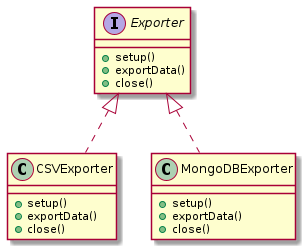
\includegraphics[width=1\linewidth]{images/alchemist-strategy.png}
	\caption{Schema della nuova interfaccia Exporter.}
	\label{fig:uml-alchemist-strategy}
\end{figure}
Nello specifico vengono realizzate le seguenti implementazioni:
\begin{itemize}
    \item \texttt{CSVExporter}: si tratta di un'estensione della classe originale \texttt{Exporter} e si occupa di esportare i dati su un file in formato \textit{CSV} compatibile con il precedente sistema.
    \item \texttt{MongoDBExporter}: si occupa di esportare i dati della simulazione sul database NoSQl \textit{MongoDB}. La classe dovrà essere in grado di esportare i dati indipendentemente dalla locazione del database: verranno eseguiti dei test sia su delle istanze del database in locale che su soluzioni in cloud.
\end{itemize}
Gli esportatori presenti nella nuova architettura svolgono un insieme di operazioni come ad esempio l'inizializzazione dell'ambiente di export che sono in realtà comuni ad entrambi.
A fronte di ciò risulta estremamente comodo creare un'implementazione astratta di un esportatore che si occupa di svolgere solo ed esclusivamente le operazioni comuni in modo da evitare inutili ripetizioni di codice.
Viene quindi creata la classe \texttt{AbstractExporter} la quale conterrà i metodi comuni a tutte le implementazioni dell'interfaccia e in particolare si occuperà di contenere gli oggetti necessari a entrambe per estrarre valori a partire dalle entità del simulatore.
Nella realizzazione della classe si è reso utile l'utilizzo del design pattern \textbf{Template Method}.
Il pattern comportamentale \textit{Template Method} viene utilizzato per definire la struttura di un algoritmo delegando alcuni passi di dettaglio alle sottoclassi.
Questo pattern nasce dall’esigenza di specificare l’ordine delle operazioni da effettuare ma di delegare alle sottoclassi l’implementazione di alcune operazioni. Pertanto il metodo che definisce l’algoritmo viene implementato nella superclasse mentre i metodi che definiscono i comportamenti di dettaglio vengono dichiarati astratti nella superclasse ed implementati nelle sottoclassi.
\begin{figure}
	\centering
	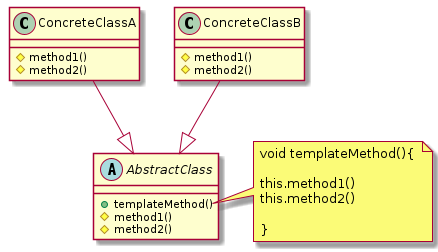
\includegraphics[width=1\linewidth]{images/template_method.png}
	\caption{Diagramma delle classi del design pattern Template Method.}
	\label{fig:uml-template_method}
\end{figure}
Questo pattern è composto dalle seguenti entità:
\begin{itemize}
    \item \textbf{AbstractClass}: definisce il metodo concreto ed i metodi primitivi astratti. Il metodo concreto richiama i metodi primitivi implementati nelle sottoclassi.
    \item \textbf{ConcreteClass}: implementa i metodi primitivi per svolgere i passi specifici dell’algoritmo ed eventualmente i metodi hook.
\end{itemize}
L'utilizzo di questo pattern consente di:
\begin{itemize}
    \item implementare una sola volta la parte ``immutata" dell’algoritmo e di consentire alle sottoclassi di implementare il comportamento delle parti “variabili”;
    \item individuare comportamenti comuni delle sottoclassi e “promuoverli” a comportamenti della superclasse in modo da evitare la duplicazione di codice: un esempio di refactoring di codice.
\end{itemize}
Attraverso il metodo template \textit{update()} la classe astratta delegherà alle sue sottoclassi l'implementazione dello stesso a seconda della tipologia di esportazione che esse rappresentano.
\begin{figure}
	\centering
	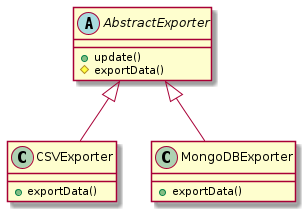
\includegraphics[width=1\linewidth]{images/alchemist-template_method.png}
	\caption{Schema del pattern Template Method della nuova architettura.}
	\label{fig:uml-abstract-exporter}
\end{figure}

A fronte del requisito funzionale di poter scegliere il tipo di esportazione direttamente nel file di configurazione, viene modifcata la sintassi della chiave \texttt{export}.
Un esempio della nuova sintassi è il seguente:\\
 \begin{minted}[
    frame=single,
    linenos,
    samepage
  ]{yaml}
export:
    - type: AlchemistClassicCSV
      parameters: 
        filename: "/my/data/folder"
        appendTime: true
      data:
        - time
        - molecule
        value-filter : onlyfinite

    - type: MongoDBExporter
      parameters: 
        uri: "mongodb@127.0.0.1:8080"
        dbName: "alchemist-test"
        interval: 2.5
      data:
        - time
        - molecule
        aggregators: [mean, max, min, variance, median]
\end{minted}
In particolare, è possibile dichiarare una lista di esportatori e, per ciascuno di essi, specificarne la tipologia.
Tra i parametri aggiunti possiamo trovare i valori dei costruttori degli esportatori come ad esempio \textit{fileNameRoot}, \textit{uri} e \textit{interval} e la chiave \textit{data} che rappresenta la sezione nella quale si dichiarano i dati da esportare. Alcuni parametri saranno opzionali in quanto avranno dei valori di default, altri invece saranno obbligatori in quanto indispensabili per poter istanziare correttamente gli esportatori.\\
La nuova interfaccia \texttt{Exporter} non viene considerata in senso stretto un \textit{boundary} dell'applicazione ossia non implementa direttamente l'interfaccia \texttt{OutputMonitor}. Le ragioni di questa scelta nascono del fatto che viene considerato come \textit{boundary} l'intero sistema di export e non ogni singolo esportatore. A fronte di ciò viene creata la classe \texttt{GlobalExporter}.
La classe implementa il boundary \texttt{OutputMonitor} e contiene al proprio interno la lista degli esportatori scelti nel file di configurazione.
Durante l'esecuzione il motore del simulatore notificherà alla classe ad ogni passo lo stato della simulazione, quest'ultima provvederà a fare eseguire l'export ad ognuno dei suoi esportatori.
La \cref{fig:uml-global-arch} mostra una visione globale della nuova architettura.

\begin{figure}
	\centering
	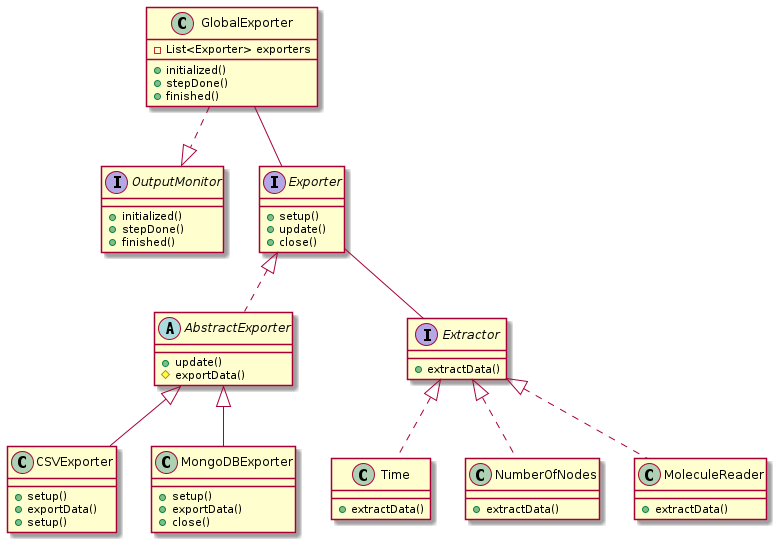
\includegraphics[width=1\linewidth]{images/alchemist-export-new.png}
	\caption{Diagramma delle classi della nuova architettura.}
	\label{fig:uml-global-arch}
\end{figure}

\subsection{Design dettagliato}
In questa sezione approfondiremo alcuni elementi di design con maggior dettaglio.

\subsubsection{Exporter}
\begin{figure}
	\centering
	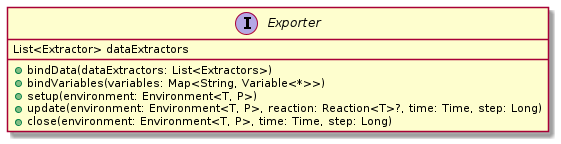
\includegraphics[width=1\linewidth]{images/exporter.png}
	\caption{Interfaccia Exporter.}
	\label{fig:exporter}
\end{figure}
In un generico esportatore per il simulatore risulta di primaria importanza contenere dei metodi per elaborare e convertire i dati forniti dalla simulazione in un formato esportabile. Tutto ciò viene svolto dall'interfaccia \texttt{Extractor}. Nello specifico l'interfaccia conterrà una serie di implementazioni a seconda della tipologia di dato da estrarre. Durante la preparazione della simulazione verrà assegnata all'esportatore una lista di estrattori tramite il metodo \texttt{bindData}. In aggiunta agli estrattori di dati verranno comunicate all'esportatore anche le variabili utilizzate tramite il metodo \texttt{bindVariables}.
La fase di preparazione dell'ambiente di esportazione viene eseguita all'interno del metodo \texttt{setup} che verrà invocato prima dell'inizio della simulazione.
Per terminare l'esportazione in modo corretto è presente il metodo \texttt{close} il quale verrà invocato al termine della simulazione.
Ad ogni passo della simulazione verrà invocato il metodo \texttt{update} nel quale la classe astratta controllerà se far esportare i dati a seconda dell'intervallo di campionamento scelto.

\subsubsection{CSVExporter}
La classe \texttt{CSVExporter} ha il compito di esportare i dati generati dalla simulazione su un file in formato CSV.
Per utilizzare questa tipologia di esportatore è possibile fornire alcune informazioni aggiuntive nel file di configurazione. 
In particolare è possibile indicare il nome del file che verrà generato grazie al parametro \texttt{fileNameRoot} e l'intervallo di campionamento tramite il parametro \texttt{interval}.
Inoltre è possibile specificare una destinazione per la cartella contenente il file di output tramite il parametro \texttt{path}. Se non viene indicata nessuna destinazione, il simulatore esporterà il file all'interno di una cartella temporanea.
Esistono scenari in cui si intende confrontare il file di output con quello della precedente esecuzione mentre in altre situazioni l'unico file di interesse è quello della simulazione più recente. Per supportare entrambi i casi viene utilizzato il parametro \texttt{appendTime}.
In relazione ai parametri scelti, la stringa finale contenente la destinazione del file di output sarà salvata nella proprietà \texttt{exportDestination}. 
All'interno del  metodo \texttt{setup()} la classe si occuperà di creare la cartella in cui generare il file se essa non è presente. Successivamente verrà istanziato un oggetto della classe \texttt{PrintStream} che avrà il compito di aprire uno stream in scrittura sul file di output. Le prime informazioni esportate riguardano i nomi delle variabili presenti nella simulazione e i nomi delle colonne dei dati che si andranno ad esportare.
Il metodo \texttt{exportData()} conterrà l'effettiva implementazione dell'esportazione dei dati sul file. Per ciascun elemento appartenente alla lista interna di estrattori verranno esportati i dati generati in relazione a i valori correnti dello step della simulazione. Nel metodo \texttt{close()} l'exporter si occuperà di scrivere sul file un messaggio contenente l'orario di fine simulazione e di terminare in modo corretto l'esecuzione dello stream in scrittura.

\begin{figure}
	\centering
	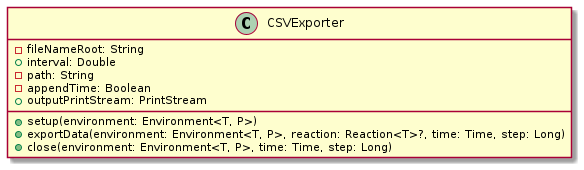
\includegraphics[width=1\linewidth]{images/csvexporter.png}
	\caption{classe CSVExporter.}
	\label{fig:csv-exporter}
\end{figure}

\subsubsection{MongoDBExporter}
    La classe \texttt{MongoDBExporter} si occupa di esportare i dati della simulazione sul database NoSQl \textit{MongoDB}.
    Se si intende utilizzare questa tipologia di esportatore è obbligatorio indicare nel file di configurazione l'indirizzo in cui è presente un istanza di \textit{Mongo} tramite il parametro \texttt{uri}.
    In aggiunta è possibile specificare il nome del database su cui esportare i dati tramite il parametro \texttt{dbName}. Se non viene indicato alcun valore verrà utilizzato il database di default chiamato \textit{test}.
    In comune con il \texttt{CSVExporter} è possibile specificare l'intervallo di campionamento con il parametro \texttt{interval} e si può scegliere se sovrascrivere i dati nel database ad ogni esecuzione con il parametro \texttt{appendTime}.
    \begin{figure}
    	\centering
    	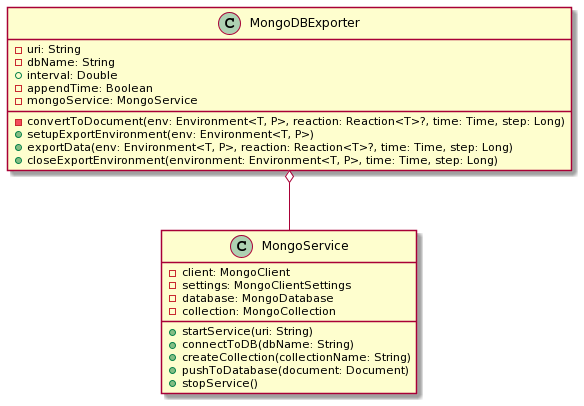
\includegraphics[width=1\linewidth]{images/mongodbexporter.png}
    	\caption{schema dell'interazione tra le classi MongoDBExporter e MongoService.}
    	\label{fig:mongo-exporter}
    \end{figure}
    Tutto ciò che riguarda il dominio di \textit{MongoDB} ossia i vari oggetti e collezioni per connettersi ed interagire con il database saranno presenti unicamente all'interno della classe \texttt{MongoService} che verrà istanziata come campo dell'esportatore.
    Nel metodo \texttt{setup()}, a partire dalla stringa di connessione, avviene la connessione al database e la creazione di una collezione che rappresenta un'insieme di documenti per la simulazione corrente. Per fare ciò, l'esportatore utilizza i metodi \texttt{startService()}, \texttt{connectToDB()} e \texttt{createCollection()} della classe \textit{MongoService}.
    Il metodo \texttt{exportData()} utilizza il metodo privato \texttt{convertToDocument()} per ottenere un documento in formato BSON\footnote{\url{https://bsonspec.org/spec.html}} ed una volta ottenuto utilizza il metodo \texttt{pushToDatabase()} del \textit{service} per aggiungere il documento alla collezione nel database.
    Il metodo privato \texttt{convertToDocument()} si occupa di generare un documento BSON a partire dalla lista interna di estrattori di dati.
    Infine nel metodo \texttt{close()} viene terminata in modo corretto l'esecuzione del \textit{service}.
    \section{Implementazione}
    L'insieme delle classi e test sviluppati si trovano sotto il modulo \textbf{alchemist-loading} del simulatore. Gli interventi eseguiti in classi al di fuori di questo modulo riguardano l'adattamento delle classi e dei test alla nuova architettura.
    
\subsection{Strumenti di sviluppo}

    \subsubsection{\textbf{Git}}
    Git\footnote{\url{https://git-scm.com/}} è un sistema di controllo di versione distribuito (DVCS) che permette di tenere traccia delle modifiche effettuate durante lo sviluppo di software. Tra le varie funzionalità, git offre la possibilità di mantenere due versioni dello stesso progetto: una stabile e una in via di sviluppo; tale organizzazione risulta piuttosto flessibile per fronteggiare i problemi che solitamente si incontrano in fase di implementazione. Alchemist è sviluppato con la metodologia di lavoro nota come Gitflow\footnote{\url{https://nvie.com/posts/a-successful-git-branching-model/}}, che prevede che ogni componente del team di sviluppo abbia una propria copia del progetto principale: l'aggiunta di codice al repository centrale avviene per mezzo di \emph{pull requests}, con le quali un membro del team richiede che il suo codice sia aggiunto a tale repository.
    Il codice è stato quindi sviluppato in una copia del repository originale e sotto il branch \textit{develop}.
    Il codice inerente allo sviluppo di un esportatore su MongoDB è stato scritto sotto il branch \textit{feature-mongo}.
    
    \subsubsection{\textbf{Gradle}}
    Gradle\footnote{\url{https://gradle.org/}} è uno strumento per l’automazione della costruzione del software, organizzato in task per semplificare la compilazione del codice sorgente, la risoluzione delle dipendenze, l’esecuzione dei test automatici e il controllo di qualità del codice. In breve, esso è in grado di determinare quali porzioni del sistema software necessitano di essere ricostruite riducendo significativamente il tempo di costruzione del progetto. Questo sistema permette di avere una gestione controllata delle dipendenze le quali vengono scaricate dai vari repository Maven\footnote{\url{https://search.maven.org/}} durante la fase di compilazione. Il simulatore Alchemist, mantiene, oltre a quello generale di progetto, uno script Gradle per ogni modulo presente al suo interno, nel quale sono specificati gli altri moduli o eventuali librerie esterne di cui si vogliono utilizzare le funzionalità.
    
    \subsubsection{GitHub CI}
    Il simulatore utilizza un sistema di \textit{Continuous Integration} per monitorare il comportamento del software allo stato attuale, installandolo ed eseguendolo su diverse macchine virtuali, con diversi sistemi operativi e diverse configurazioni.
    Questa possibilità, permette di tenere sempre sotto controllo la retrocompatibilità ed il supporto multi-piattaforma del simulatore, testandone il funzionamento con diverse versioni della JVM su tutti i principali sistemi operativi. L'intero processo è configurabile attraverso un file YAML e viene eseguito ad ogni push sul repository.
    
    \subsubsection{\textbf{Kotlin}}
    Tutte le classi sviluppate sono state scritte in Kotlin\footnote{\url{https://kotlinlang.org}}, un linguaggio di programmazione open-source.
    La sua principale caratteristica è quella di essere pienamente interoperabile con il linguaggio Java e la Java Virtual Machine (JVM) e cioè di poter sfruttare tutte le librerie presenti per Java e al contempo di poter essere importato all’interno di codice Java senza riscontrare particolari problemi.
    Kotlin è un linguaggio multi-paradigma, in quanto presenta sia caratteristiche tipiche della programmazione orientata agli oggetti sia del paradigma funzionale, e multi-piattaforma, poiché, oltre che per la JVM, può essere compilato per Android, iOS, JavaScript e nativamente per Windows, Linux e MacOS.
    La scelta dell’uso di Kotlin al posto di Java per l’implementazione degli esportatori all’interno di Alchemist, si è rilevata molto utile in diversi frangenti, nei quali altrimenti, per ottenere lo stesso risultato, si sarebbe dovuto adottare soluzioni molto più verbose e di difficile comprensione. Un esempio di ciò lo si può notare nei costruttori degli esportatori. Grazie all'utlizzo della notazione \texttt{@JVMOverloads} verrà generata, per ogni parametro di default, l’overload della funzione. Per ottenere lo stesso risultato in Java sarebbe stato necessario creare molteplici costruttori, in particolare uno per ciascuna combinazione di parametri.
    
    \subsubsection{Librerie esterne}
    Durante lo sviluppo del progetto, in particolare nell'implementazione dell'esportatore per il database MongoDB è stata utilizzata la libreria \textbf{mongo-driver-sync}\footnote{\url{https://search.maven.org/artifact/org.mongodb/mongodb-driver-sync/3.10.1/jar}}.
    La libreria contiene i driver del database Mongo per il linguaggio Java ossia un insieme di metodi per aiutare lo sviluppatore a connettersi ed interagire con il database.
    Gli oggetti e le strutture dati fornite dalla libreria, come ad esempio \textit{MongoClient}, \textit{MongoCollections} e \textit{MongoDatabase} sono risultati estramamente utili in termini di efficienza e pulizia del codice.
    
\subsubsection{Valutazione del codice}
    Date le dimensioni di Alchemist, è necessario fare uso di strumenti che controllino la qualità del codice e diano la possibilità di testarlo in modo immediato. Gli strumenti di qualità del codice permettono di revisionare il codice in modo sistematico, così da evitare errori che a volte possono verificarsi, senza bisogno che il programma
    venga realmente eseguito: essi analizzano il codice sorgente per individuare potenziali bug
    o codice duplicato e per indicare i possibili miglioramenti e ottimizzazioni.
    Alchemist utilizza i seguenti strumenti:
    \begin{itemize}
        \item \textbf{checkstyle}: è uno strumento open-source per diversi linguaggi di programmazione e verifica che il codice scritto aderisca a un determinato stile di codifica. Esso effettua un controllo sulla presentazione e non sul contenuto, dunque non permette di assicurare la correttezza e la completezza del software.
        \item \textbf{detekt}: è uno strumento open-source di analisi del codice per il linguaggio Kotlin.Prevede un set di regole, personalizzabile dallo sviluppatore, per definire quando una parte del codice è errata.
        \item \textbf{pmd}: è uno strumento di analisi del codice sorgente per Java e altri linguaggi.
        Generalmente, gli errori segnalati riguardano scelte implementative subottimali e imperfezioni nel codice, che non inficiano direttamente il funzionamento del programma ma per la maggior parte il livello della qualità del sorgente.
        \item \textbf{ktlint}: è uno strumento di analisi del codice sorgente per il linguaggio Kotlin. Contiene delle regole standard ma offre anche la possibilità di aggiungere un file di configurazione contente le regole da rispettare.
        \item \textbf{spotbugs}: è uno strumento open-source che opera direttamente sul bytecode Java e rileva possibili bug all'interno del codice. Classifica i potenziali errori in categorie, per dare un’idea migliore allo sviluppatore di quale potrebbe essere il loro impatto sul software.
        \item \textbf{cpd}: è un plugin che analizza il codice sorgente con lo scopo di ricerca di codice duplicato.
    \end{itemize}
    
\subsubsection{Ambiente di sviluppo integrato}
    Un IDE (Integrated Development Environment), o ambiente di sviluppo integrato, è un software che aiuta i programmatori nello sviluppo del codice sorgente di un programma, mettendo a disposizione una serie di strumenti che permettono scrittura, compilazione o interpretazione, debug e analisi del codice da un unico ambiente, appunto, integrato.
    Durante lo sviluppo è stato utilizzato l'ambiente di sviluppo \textbf{IntelliJ IDEA}\footnote{\url{https://www.jetbrains.com/idea/}}, sviluppato da JetBrains, nell'edizione \textit{ultimate}.
    
\subsection{Testing}
    In parallelo alla fase di sviluppo è stata portata avanti un’attività di Unit testing per ogni nuova funzionalità introdotta, con lo scopo di verificarne il corretto funzionamento e impedendo così che nuove modifiche introdotte nel simulatore possano compromettere il suo stato di avanzamento attuale.
    Per la creazione dei test sono state utilizzate le librerie \textit{Kotest}\footnote{\url{https://kotest.io/}} e \textit{JUnit}\footnote{\url{https://junit.org/junit5/}}, grazie alle quali è stato possibile testare dei comportamenti in un linguaggio simile al naturale.
    Ciascun test effettuato è stato affiancato da un opportuno file di configurazione in formato YAML. In questo modo è stato possibile lanciare simulazioni e testare le varie fasi di interesse.
    In particolare, all'interno della classe \textbf{TestExportersCreation} a partire da un file di configurazione in cui venivano dichiarati molteplici esportatori, è stato testato il corretto caricamento degli stessi e per ciascuno di essi sono state testate le strutture dati necessarie. 
    Un'altra funzionalità della quale è necessario verificare la corretta esecuzione è l'esportazione su file. Partendo da un file di configurazione in cui veniva dichiarato un \textit{CSVExporter} nella classe \textbf{TestCSVExporter} è stata testata la corretta appartenenza alla classe e la presenza del file di output generato.
    La nuova architettura permette di specificare intervalli di campionamento differenti a seconda della tipologia di esportatore. Questa funzionalità è stata testata all'interno della classe \textbf{TestExportInterval}.
    Per quanto riguarda l'esportazione su database è necessario testare inizialmente se è presente un'istanza attiva del database. Nello specifico, nella classe \textbf{TestMongoInstance} viene testato il corretto funzionamento della libreria \texttt{embedded-mongodb} ossia se è presente un processo di mongodb in locale e in caso affermativo se è possibile connettersi ed interagire con il database. 
    Per quanto riguarda invece l'esportatore \textit{MongoDBExporter}, nella classe \textbf{TestMongoDBExporter} viene testata la connessione al database MongoDB con i parametri forniti nel file di configurazione. Inoltre è stata testata la creazione del database e l'effettiva presenza dei dati esportati in esso.
    \begin{figure}
	\centering
	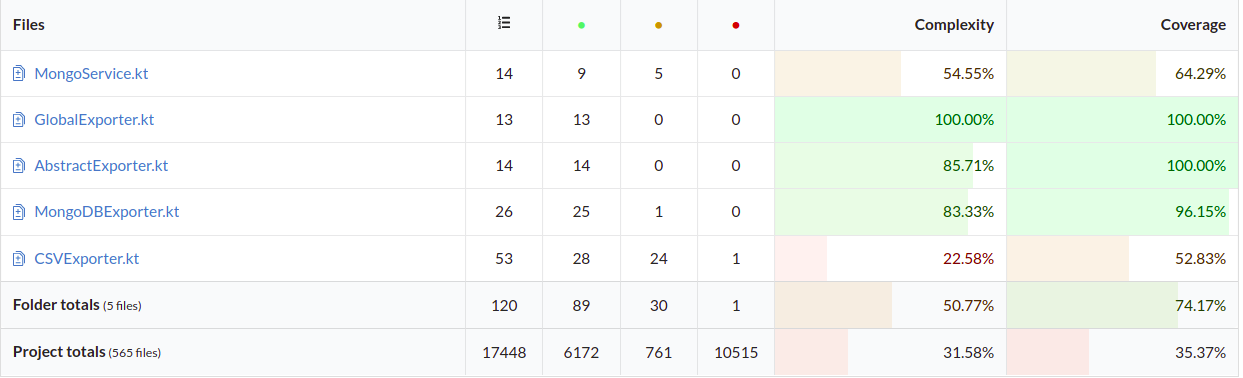
\includegraphics[width=1\linewidth]{images/coverage.png}
	\caption{Coverage del codice sviluppato.}
	\label{fig:code-coverage}
    \end{figure}
    
\chapter{Conclusioni e sviluppi futuri }

\section{Conclusioni}
    Lo scopo di questo lavoro era quello di analizzare il dominio della generazione di dati tramite simulazione, analizzare lo stato dell'arte e infine applicare quanto appreso nella ri-progettazione di un modulo di esportazione dati per il simulatore Alchemist.
    A lavoro terminato possiamo affermare che l'architettura precedente ha subito notevoli modifiche. Tra i cambiamenti più rilevanti troviamo:
    \begin{itemize}
        \item possibilità di scegliere la tipologia di esportazione direttamente nel file di configurazione;
        \item eliminazione dei parametri \textit{export} ed \textit{interval}: l'utente non dovrà più specificare il nome del file e l'intervallo di campionamento come parametri della simulazione ma verranno indicati opportunamente nel file di configurazione;
        \item creazione di un'interfaccia di export e di una classe astratta contenente i metodi comuni a tutti gli esportatori;
        \item sviluppo di un esportatore verso il database \textit{MongoDB}.
    \end{itemize} 
    
\section{Sviluppi futuri}
    Una delle principali caratteristiche del nuovo sistema di export riguarda sicuramente la flessibilità e la dinamicità con cui possono essere aggiunti nuovi esportatori.
    In particolare, sarà necessario solamente estendere la classe \texttt{AbstractExporter} ed implementare il metodo principale per esportare i dati. Una volta creata basterà aggiungere il nome della nuova classe dell'esportatore nel file di configurazione e il sistema lo aggiungerà in automatico alla lista di esportatori presenti.
    Il lavoro potrà quindi essere esteso aggiungendo delle nuove tipologie di esportatori come ad esempio un'implementazione per un differente database oppure un esportatore responsabile di creare grafici in tempo reale con i dati generati dalla simulazione.

\bibliographystyle{plain}
\bibliography{bibliography}
\addcontentsline{toc}{chapter}{Bibliografia}

\chapter*{Ringraziamenti}
\addcontentsline{toc}{chapter}{Ringraziamenti}
    Un sincero ringraziamento va a tutti coloro che mi hanno aiutato in vario modo a raggiungere questo traguardo.\\
    Ringrazio tutti i professori del corso di studi in Ingegneria e Scienze Informatiche, che mi hanno trasmesso grande passione per le loro materie. \\
    In particolar modo, ringrazio il professor Danilo Pianini e il professor Mirko Viroli per l'opportunità che mi hanno concesso e per le numerose nozioni apprese durante il progetto.\\
    Ringrazio i miei genitori ed i miei amici, che mi hanno supportato incondizionatamente durante il  percorso.\\
    Ringrazio infine i miei compagni di studio, con i quali ho condiviso tre bellissimi anni e che sono stati una spalla su cui contare dall'inizio alla fine della mia carriera universitaria.

\appendix
\chapter{Esempi di file di simulazioni}

\section{Sezione di export con CSVExporter}
 \begin{minted}[frame=single]{yaml}
export:
  - type: CSVExporter
    parameters: 
      filename: "00-testing_csv_export"
      appendTime: true
      interval: 2.0
    data:
      - time
      - molecule: "default_module:default_program"
        aggregators: [ mean, max, min, variance, median ]
        value-filter: onlyfinite
\end{minted}
\section{Sezione di export con MongoDBExporter}
 \begin{minted}[frame=single]{yaml}
 export:
  - type: MongoDBExporter
    parameters:
      uri: "mongodb+srv://alchemist-user:alchemist-pwd
           @alchemist.ewxds.mongodb.net"
      appendTime: false
      dbname: "alchemist-mongo-test"
      interval: 3.0
    data:
      - time
      - molecule: "default_module:default_program"
        value-filter: onlyfinite
\end{minted}
\section{Sezione di export con più esportatori}
 \begin{minted}[frame=single]{yaml}
 export:
  - type: CSVExporter
    parameters: 
      filename: "00-testing_csv_export"
      appendTime: true
      interval: 2.0
    data:
      - time
        
  - type: MongoDBExporter
    parameters:
      uri: "mongodb+srv://alchemist-user:alchemist-pwd
           @alchemist.ewxds.mongodb.net"
      appendTime: false
      dbname: "alchemist-mongo-test"
      interval: 3.0
    data:
      - time
      - molecule: "default_module:default_program"

\end{minted}
\section{Simulazione di esempio completa}
 \begin{minted}[frame=single]{yaml}
 incarnation: protelis
variables:
  zoom: &zoom
    formula: 0.1
  image_name: { formula: "'chiaravalle.png'" }
  image_path: &image_path
    language: kotlin
    formula: >
      import java.io.File
      File("../..").walkTopDown().find { 
      image_name in it.name
      }?.absolutePath ?: image_name
  walking_speed: &walk-speed { 
    default: 1.4, min: 1, max: 2, step: 0.1 }
  seed: &seed { default: 0, min: 0, max: 99, step: 1 }
  scenario_seed: &scenario_seed { formula: (seed + 31) * seed }
  people_count: &people_count
    type: GeometricVariable
    parameters: [300, 50, 500, 9]
seeds: { simulation: *seed, scenario: *scenario_seed}
export:
  - type: CSVExporter
    parameters: 
      filename: "00-testing_csv_export"
      appendTime: false
      interval: 2
    data:
      - time
        aggregators: [ mean, max, min, variance, median ]

  - type: MongoDBExporter
    parameters:
      uri: "mongodb+srv://alchemist-user:alchemist-pwd
            @alchemist.ewxds.mongodb.net"
      dbname: "alchemist-testing-mongo"
      interval: 3.0
    data:
      - molecule: "default_module:default_program"
        value-filter: onlyfinite      
        
environment: { type: ImageEnvironment,
               parameters: [*image_path, *zoom] }
network-model: { type: ObstaclesBreakConnection,
                 parameters: [50] }
deployments:
  type: Rectangle
  parameters: [*people_count, 62, 15, 95, 200]
  programs:
    - time-distribution: 1
      program: >
        import protelis:coord:spreading
        let source = [110, 325]
        let vector = self.getCoordinates() - source
        let distance = hypot(vector.get(0), vector.get(1))
        distanceTo(distance < 50)
    - program: send
    - { type: Event, time-distribution: 1, actions: { 
        type: LevyWalk, parameters: [*walk-speed] } }

terminate:
  - type: AfterTime
    parameters: 5
\end{minted}

\end{document}
